% 18 variables in here:
% h_1 = 1000.0, h_2 = 1002.0, h_3 = 997.0, h_4 = 1005.0, h_5 = 1001.0, h_6 = 999.0, ux_1 = -1.0, ux_2 = 2.0, ux_3 = -3.0, ux_4 = 4.0, ux_5 = -5.0, ux_6 = 6.0, uy_1 = 1.0, uy_2 = -2.0, uy_3 = 3.0, uy_4 = -4.0, uy_5 = 5.0, uy_6 = -6.0
\begin{figure}[h!]
\centering
  \subfigure[] {
    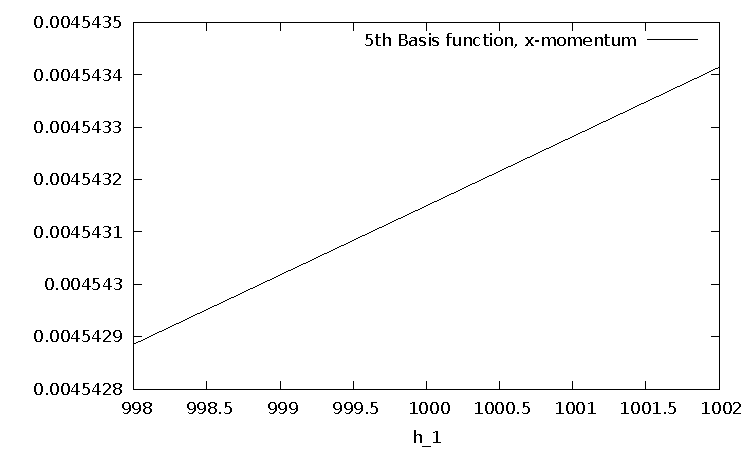
\includegraphics[scale=\zoomfactor]{{{ord2_magnitude_comparison_1000_heights_momentums/y_1002.0_997.0_1005.0_1001.0_999.0_-1.0_2.0_-3.0_4.0_-5.0_6.0_1.0_-2.0_3.0_-4.0_5.0_-6.0f08}}}
  }
  \subfigure[] {
    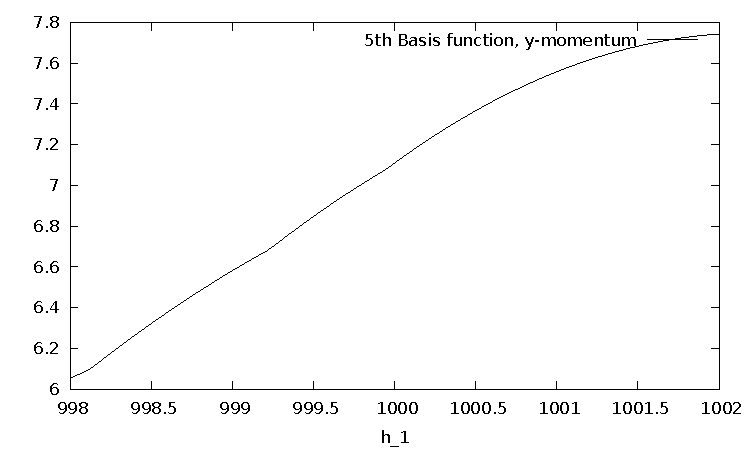
\includegraphics[scale=\zoomfactor]{{{ord2_magnitude_comparison_1000_heights_momentums/y_1002.0_997.0_1005.0_1001.0_999.0_-1.0_2.0_-3.0_4.0_-5.0_6.0_1.0_-2.0_3.0_-4.0_5.0_-6.0f09}}}
  }
\caption{}
\label{fig:ord2_magnitude_comparison_1000_momentum}
\end{figure}

%%% Local Variables:
%%% TeX-master: "../results.tex"
%%% End:
